\documentclass[titlepage,a4paper,10pt]{article}
% Språk och encodings
\usepackage[swedish,english]{babel}
\usepackage[T1]{fontenc}
\usepackage[utf8]{inputenc}
\usepackage[fixlanguage]{babelbib}
% Images and floats
\usepackage{graphicx}
\usepackage{wrapfig}
\usepackage{float}
% Clear type + Sans-serif font
\usepackage{lmodern}
\renewcommand{\familydefault}{\sfdefault}
% Matte
\usepackage{amsmath, amsthm, amssymb}
% Algoritmer
\usepackage[ruled,vlined]{algorithm2e}
% Länkar
\usepackage{color}
\definecolor{dark-blue}{rgb}{0, 0, 0.6}
\usepackage{hyperref}
\hypersetup{
  colorlinks=true,
  linkcolor=dark-blue,
  urlcolor=dark-blue
}
% Vettiga paragrafer
\setlength{\parindent}{0pt}
\setlength{\parskip}{2ex}

% Sidhuvud/sidfot
\usepackage{fancyhdr}
\setlength{\headheight}{15pt}
\pagestyle{fancyplain}
\lfoot{Carl-Oscar Erneholm \\ 880422-0872 \\ coer@kth.se}
\rfoot{Martin Nycander \\ 881028-0076 \\ mnyc@kth.se}
\cfoot{Page \thepage}

% Språk
\selectbiblanguage{swedish}
\selectlanguage{swedish}

% Titel
\title{ID1217: Parallel Particle Simulation}
\author{Martin Nycander \and Carl-Oscar Erneholm}
\date{\today}

\begin{document}
\maketitle

\tableofcontents
\newpage

\setcounter{page}{1}
% In your report you should explain what you have done and what you have learned.
% Your report should be few (about 10) pages of text plus tables and figures and an optional Appendix.

\section{Problem definition}




The problem is to optimize and parallelize a particle simulator, we
were given four implementations of the simulator:

\begin{wrapfigure}{r}{0.3\textwidth}
    \vspace{-130pt}
    \begin{center}
        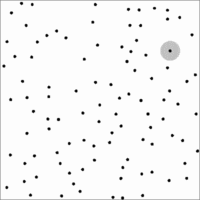
\includegraphics[width=0.28\textwidth]{simulator}
    \end{center}
    \caption{An example simulation in the provided visualizer application.}
\end{wrapfigure}

\begin{itemize}
     \item One running sequentially
     \item One parallelized using pthreads
     \item One parallelized using openmp 
     \item One parallelized using MPI
\end{itemize}

The given simulator implementation used $n^2$ computations each frame, where $n$ is the number of particles.

In contrast to the traditional N-body problem this simulation only
simulates the interaction between particles within a certain distance from
each other, moreover the density of particles is set low enough so that
only $O(n)$ interactions are expected at any given moment. Therefore it
should be possible to do the necessary calculations for each frame in
$O(n)$. The first task at hand is to make this optimization, since the given code runs in $O(n^2)$.

The second task is to use different parallelizing techniques to achieve a near optimal speedup factor. In other words, the program should run in $O(n)/T$ time, where $T$ is the number of threads.


\section{Problem solutions}


%TODO: describe how we made the serial program O(n), talk about grids.
    \subsection{Simulation Design}

        Every frame in the original implementation made $n^2$ computations. For
        each particle it calculated the distance to each other particle, if the
        particle was within the cutoff range it would also calculate and apply
        the appropriate force to the particle. The problem with this is that the
        checks the distance to all other particles when clearly not all of them
        are relevant. The solution we used was to divide the plane into a grid
        of squares, we then mapped each particle to a cell in the grid. By
        making sure that the sides of the cells is not less than the cutoff
        range, we can be sure that all relevant particles to a given particle
        are within the eight adjacent grid 


        \begin{equation}
            gridSize = \frac{\sqrt{0.0005 \cdot n}}{0.01} + 1 \\
        \end{equation}
        \begin{equation}
            grid.size = gridSize^2 = \left(\frac{\sqrt{0.0005 \cdot n}}{0.01} + 1\right)^2
        \end{equation}

    \subsection{Parallelization Design with Shared Memory}% TODO: A description of the synchronization you used in the shared memory implementation.

    \subsection{Parallelization Design with Distributed Memory}% TODO: A description of the communication you used in the distributed memory implementation.

    %Maybe this does not need its own seciton? TODO
    \subsection{Design Decisions}% TODO: A description of the design choices that you tried and how did they affect the performance.


\section{Results}

% TODO: A plot in log-log scale that shows that your serial and parallel codes run in O(n) time and a description of the data structures that you used to achieve it. In order to get more precise timing estimates, we recommend you to run a program at least 5 times and take the median (rather than the mean) of the simulation times.

\subsection{Linear execution}

In order to know that we have achieved the desired result of linear execution we
had to plot the running time against the size of the input. To to this we made a
script which automated the process and outputted vectorized plots using
\texttt{gnuplot}. The data points are the median value of $20$ simultaneous runs
on a computer in the data lab \texttt{s1810.it.kth.se} for the interval $10 \leq
n < 2000$ with a stepping of $10$ particles.

The result for our serial program can be seen in the figure below which has a
logaritmic scale, and as we can see it increases linearly.

\begin{figure}[H]
	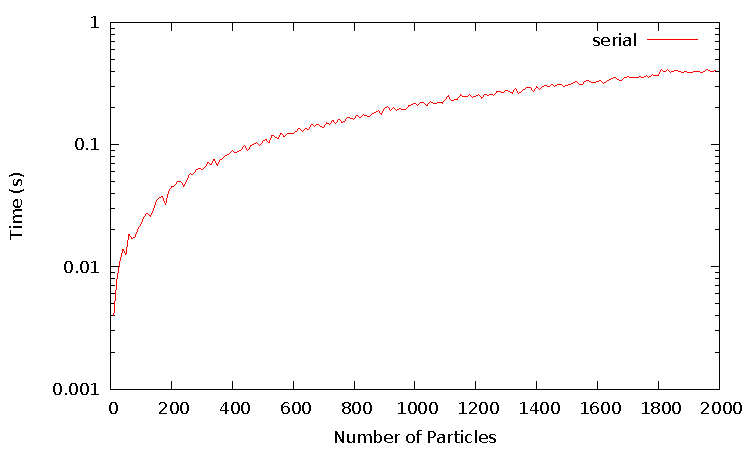
\includegraphics{plots/serial.pdf}
	\label{serial_linear}
	\caption{Execution time plotted against input size of $n$ for the serial implementation.}
\end{figure}

Our memory-shared parallel programs also proved to have linear execution when running on one thread as can be seen in the figures below.

\begin{figure}[H]
	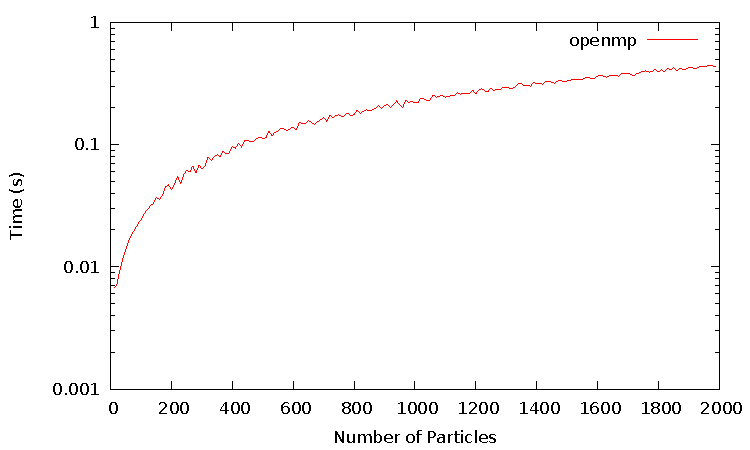
\includegraphics{plots/openmp.pdf}
	\label{openmp_linear}
	\caption{Execution time plotted against size of $n$ for the OpenMP implementation.}
\end{figure}
\begin{figure}[H]
	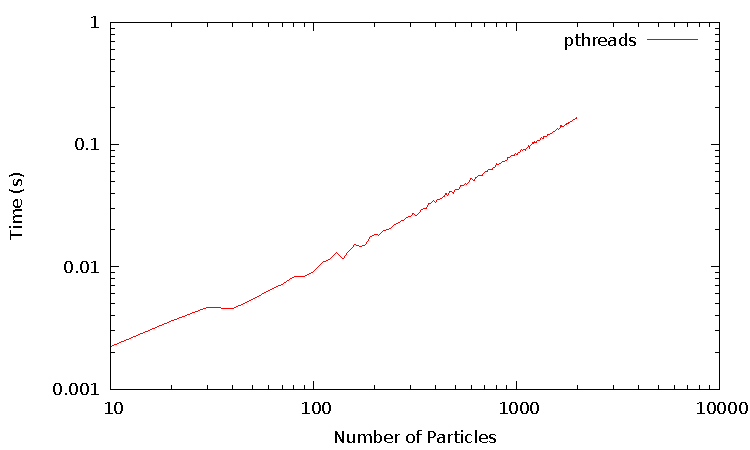
\includegraphics{plots/pthreads.pdf}
	\label{pthreads_linear}
	\caption{Execution time plotted against size of $n$ for the POSIX-threads implementation.}
\end{figure}

\begin{figure}[H]
	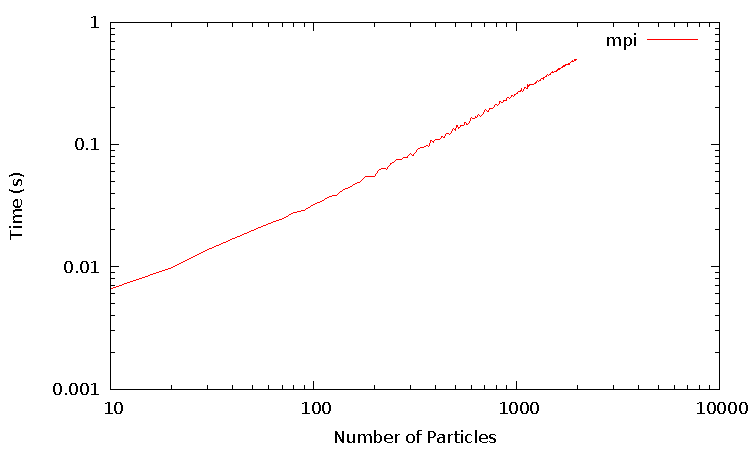
\includegraphics{plots/mpi.pdf}
	\label{mpi_linear}
	\caption{Execution time plotted against size of $n$ for the MPI implementation.}
\end{figure}

\subsection{Optimal parallelization}

The second part of the problem was to parallelize the code so that the running
time would be $O(n) / T$, where $n$ is the number of particles and $T$ is the
number of threads.

The best way to measure the level of parallelization in a program is to examine
the speedup factor. This is done by running the program with a fixed number of
threads for a number of times, extracting the median value of that and then
dividing the time with the time it took for one thread to run. The plots of the
OpenMP implementation and the POSIX-threads implementation can be seen below;
and as we can see the speedup-factor is close to optimal, but not quite.

The reason for this is a number of factors. But the major factor is that in
order for our grid optimization to work we must update the position of each
particle inside the grid. This work runs in $O(k \cdot n)$ for every thread and
in order to have optimal speed-up $k$ must be very low. However, in our case
this linear work shows through already after $2$ threads. But this critical
section of the code is required for our choice of design.

% TODO: Speedup plots that show how closely your parallel codes approach the
% idealized p-times speedup and a discussion on whether it is possible to do
% better.
\begin{figure}[H]
	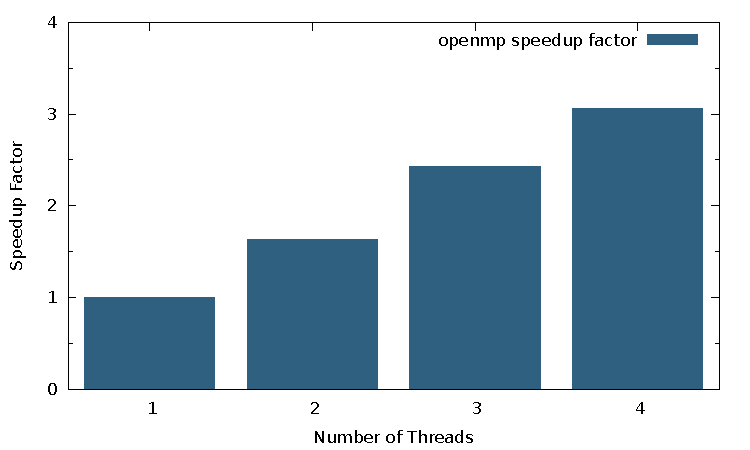
\includegraphics{plots/openmp_speedup.pdf}
	\caption{Speedup factor calculated on the \texttt{s1810.it.kth.se} computer for the OpenMP implementation.}
\end{figure}
\begin{figure}[H]
	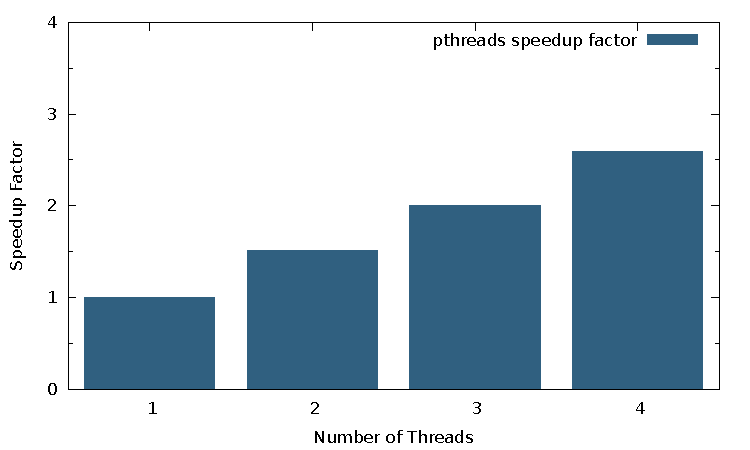
\includegraphics{plots/pthreads_speedup.pdf}
	\caption{Speedup factor calculated on the \texttt{s1810.it.kth.se} computer for the POSIX-threads implementation.}
\end{figure}

% TODO: Where does the time go? Consider breaking down the runtime into
% computation time, synchronization time and/or communication time. How do
% they scale with p?

\subsection{Problems with MPI}

The MPI implementation was by far the hardest of to get efficient, sadly we
wheren't able to get it as efficient as we hoped. Message passing is by its
nature slower than shared memory. While threads using shared memory always has
the same information as all other threads, message passing has no shared memory
and must therefore send messages in order to share information, this of course
takes extra time. The breakdown (figure 8) of our MPI implementation shows that
the computation time of the movement of the particles (move and force) follows
the near optimal speedup just as well as the other implementations. But when we
run multiple processes in MPI the message passing takes about 0.4 seconds, this
is a significant fraction of the whole execution time. When running with four
processes the message passing stands for 37\% of the computation time.
Unfortunately we could not find a way to remove this overhead. The message
passing will take up a more and more significant fraction of the computation
time because the real computation will less and less time as more processes are
added.

\begin{figure}[H]
    \label{breakdown}
	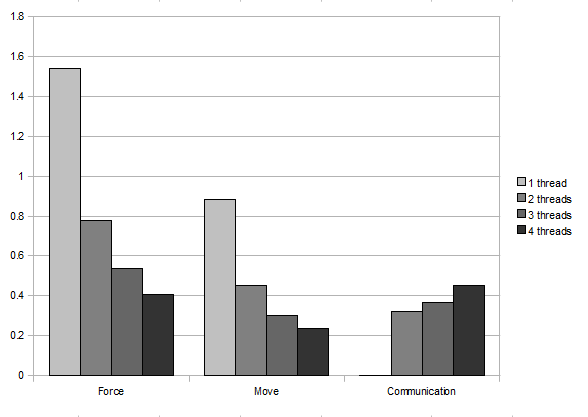
\includegraphics[width=\textwidth]{mpilol}
	\caption{Breakdown of what time is spent on when running the MPI
    implementation.}
\end{figure}


\section{Discussion}

% TODO: A plot in log-log scale that shows that your serial and parallel codes run in O(n) time and a description of the data structures that you used to achieve it. In order to get more precise timing estimates, we recommend you to run a program at least 5 times and take the median (rather than the mean) of the simulation times.

\subsection{Linear execution}

In order to know that we have achieved the desired result of linear execution we
had to plot the running time against the size of the input. To to this we made a
script which automated the process and outputted vectorized plots using
\texttt{gnuplot}. The data points are the median value of $20$ simultaneous runs
on a computer in the data lab \texttt{s1810.it.kth.se} for the interval $10 \leq
n < 2000$ with a stepping of $10$ particles.

The result for our serial program can be seen in the figure below which has a
logaritmic scale, and as we can see it increases linearly.

\begin{figure}[H]
	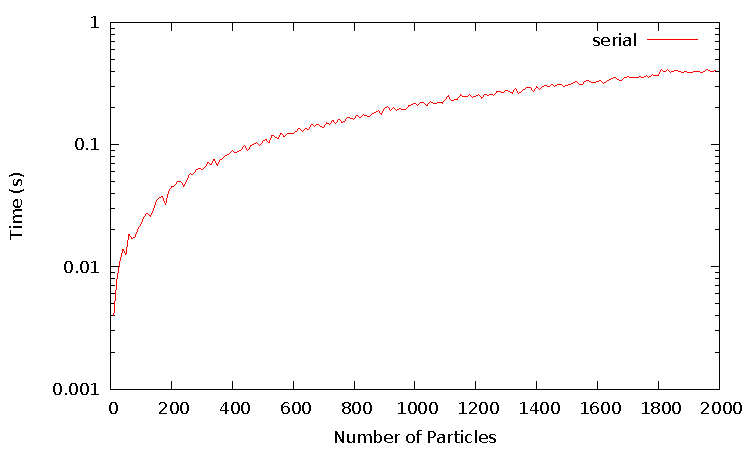
\includegraphics{plots/serial.pdf}
	\label{serial_linear}
	\caption{Execution time plotted against input size of $n$ for the serial implementation.}
\end{figure}

Our memory-shared parallel programs also proved to have linear execution when running on one thread as can be seen in the figures below.

\begin{figure}[H]
	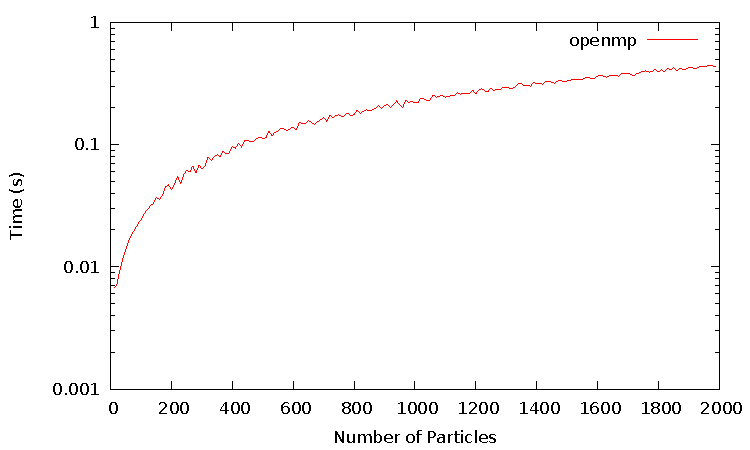
\includegraphics{plots/openmp.pdf}
	\label{openmp_linear}
	\caption{Execution time plotted against size of $n$ for the OpenMP implementation.}
\end{figure}
\begin{figure}[H]
	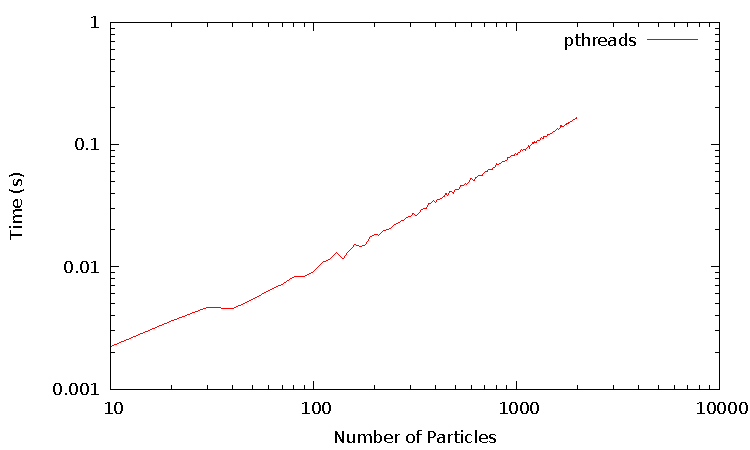
\includegraphics{plots/pthreads.pdf}
	\label{pthreads_linear}
	\caption{Execution time plotted against size of $n$ for the POSIX-threads implementation.}
\end{figure}

\begin{figure}[H]
	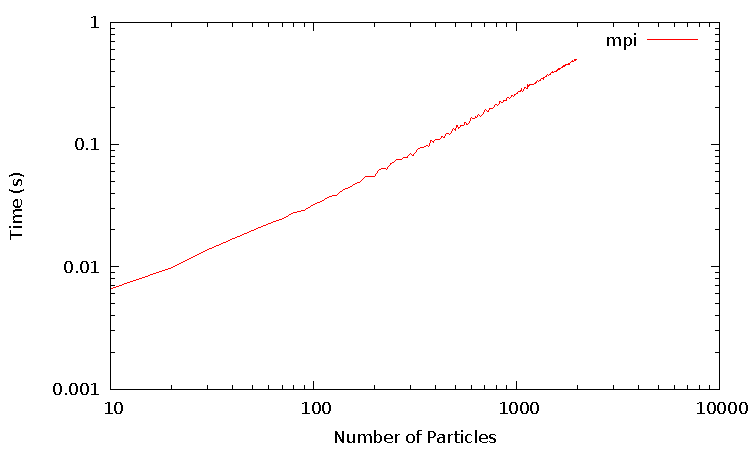
\includegraphics{plots/mpi.pdf}
	\label{mpi_linear}
	\caption{Execution time plotted against size of $n$ for the MPI implementation.}
\end{figure}

\subsection{Optimal parallelization}

The second part of the problem was to parallelize the code so that the running
time would be $O(n) / T$, where $n$ is the number of particles and $T$ is the
number of threads.

The best way to measure the level of parallelization in a program is to examine
the speedup factor. This is done by running the program with a fixed number of
threads for a number of times, extracting the median value of that and then
dividing the time with the time it took for one thread to run. The plots of the
OpenMP implementation and the POSIX-threads implementation can be seen below;
and as we can see the speedup-factor is close to optimal, but not quite.

The reason for this is a number of factors. But the major factor is that in
order for our grid optimization to work we must update the position of each
particle inside the grid. This work runs in $O(k \cdot n)$ for every thread and
in order to have optimal speed-up $k$ must be very low. However, in our case
this linear work shows through already after $2$ threads. But this critical
section of the code is required for our choice of design.

% TODO: Speedup plots that show how closely your parallel codes approach the
% idealized p-times speedup and a discussion on whether it is possible to do
% better.
\begin{figure}[H]
	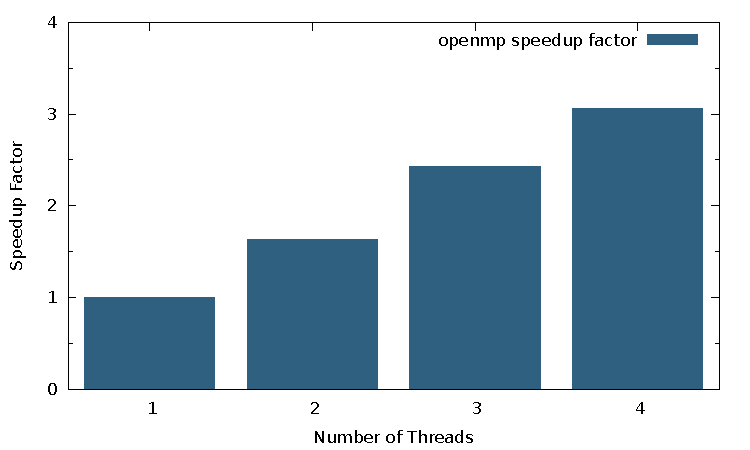
\includegraphics{plots/openmp_speedup.pdf}
	\caption{Speedup factor calculated on the \texttt{s1810.it.kth.se} computer for the OpenMP implementation.}
\end{figure}
\begin{figure}[H]
	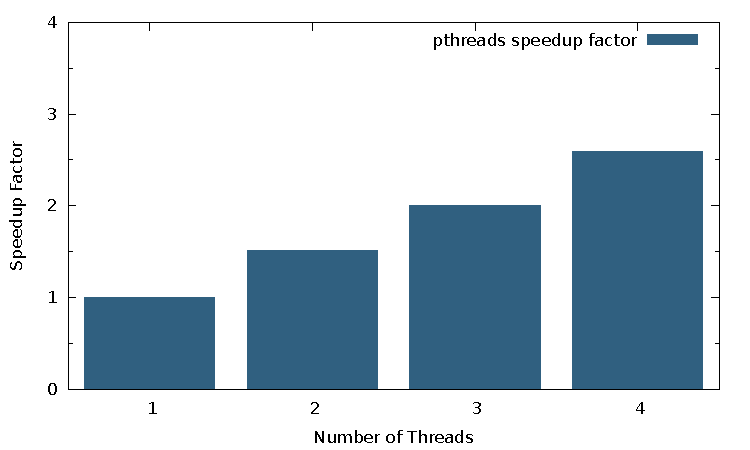
\includegraphics{plots/pthreads_speedup.pdf}
	\caption{Speedup factor calculated on the \texttt{s1810.it.kth.se} computer for the POSIX-threads implementation.}
\end{figure}

% TODO: Where does the time go? Consider breaking down the runtime into
% computation time, synchronization time and/or communication time. How do
% they scale with p?

\subsection{Problems with MPI}

The MPI implementation was by far the hardest of to get efficient, sadly we
wheren't able to get it as efficient as we hoped. Message passing is by its
nature slower than shared memory. While threads using shared memory always has
the same information as all other threads, message passing has no shared memory
and must therefore send messages in order to share information, this of course
takes extra time. The breakdown (figure 8) of our MPI implementation shows that
the computation time of the movement of the particles (move and force) follows
the near optimal speedup just as well as the other implementations. But when we
run multiple processes in MPI the message passing takes about 0.4 seconds, this
is a significant fraction of the whole execution time. When running with four
processes the message passing stands for 37\% of the computation time.
Unfortunately we could not find a way to remove this overhead. The message
passing will take up a more and more significant fraction of the computation
time because the real computation will less and less time as more processes are
added.

\begin{figure}[H]
    \label{breakdown}
	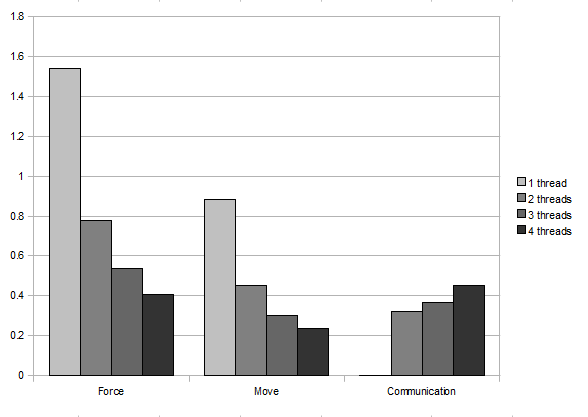
\includegraphics[width=\textwidth]{mpilol}
	\caption{Breakdown of what time is spent on when running the MPI
    implementation.}
\end{figure}


\end{document}
